\documentclass{book}

\usepackage{graphicx}

\usepackage{hyphenat} % http://www.ctex.org/documents/packages/special/hyphenat.pdf

\usepackage{setspace}\onehalfspacing\frenchspacing\flushbottom\sloppy

% https://www.scivision.dev/include-svg-vector-latex/
%\usepackage{svg}
% see https://tex.stackexchange.com/questions/442077/is-it-possible-to-use-svg-images-with-overleaf

% https://tex.stackexchange.com/a/8459/235813
\usepackage[nottoc]{tocbibind}

\usepackage{hyperref}
\hypersetup{
    colorlinks=true,
    linkcolor=blue,
    filecolor=magenta,      
    urlcolor=cyan,
    pdftitle={Overleaf Example},
    pdfpagemode=FullScreen,
    }

% https://en.wikibooks.org/wiki/LaTeX/Glossary says
% "\usepackage{glossaries} and \makeglossaries in your preamble (after \usepackage{hyperref} if present)"

% https://www.overleaf.com/learn/latex/Glossaries
\usepackage[toc]{glossaries}

\makeglossaries % The command must be before the first glossary entry.

% https://en.wikibooks.org/wiki/LaTeX/Glossary says
% "define any number of \newglossaryentry and \newacronym glossary and acronym entries in your preamble"
% see https://en.wikibooks.org/wiki/LaTeX/Glossary
% and https://www.overleaf.com/learn/latex/Glossaries

\newglossaryentry{organization}{
  name={organization},
  plural={organizations},
  description={an assembly of teams. The name of the concept might be a corporation, an agency, a department, a bureau, or any other aggregation of smaller organizations}
}

\newglossaryentry{culture}{
name={culture},
plural={cultures},
description={norms, expectations around interaction among people}
}

\newglossaryentry{stakeholder}{
name={stakeholder},
plural={stakeholders},
description={a person who cares about the process or the outcome; distinct from a participant}
%descriptionplural={people who cares about the process or the outcome; distinct from participants}
}

\newglossaryentry{participant}{
name={participant},
description={a person who is expected to take action or make contribution}
}

\newglossaryentry{essential bureaucracy}{
name={essential bureaucracy},
text={Essential bureaucracy},
description={the minimum processes and staffing and skills necessary to address the complexity of the problem space}
}

\newglossaryentry{bureaucratic debt}{
name={bureaucratic debt},
plural={bureaucratic debts},
text={Bureaucratic debt},
description={the cost of work need to change a process caused by choosing an easy solution now instead of using a better approach that would take longer}
}

\newglossaryentry{subject}{
    name={subject},
    plural={subjects},
    description={the person experiencing bureaucracy}
}
\newglossaryentry{Prisoner's dilemma}{
    name={Prisoner's dilemma},
    description={Two or more people with incomplete information of a situation will make suboptimal choices compared to someone with perfect knowledge of the situation}
}

\newglossaryentry{thought terminating}{
name={thought terminating},
description={\href{https://en.wikipedia.org/wiki/Thought-terminating_clich\%C3\%A9}{thought terminating statements} initially sound reasonable but, upon reflection and analysis, are incorrect}
}

\newglossaryentry{presence creates priority}{
name={presence creates priority},
description={being physically at a person's desk motivates that person to respond better than calling them or emailing them}
}

% https://graphthinking.blogspot.com/2021/07/bureaucracy-book-outline.html
\newglossaryentry{bureaucrat}{
    name={bureaucrat},
    plural={bureaucrats},
    description={the person who is a member of an organization and is responsible for subjective implementation of policy for the organization. Conventional examples of a bureaucrat role: teacher, police, government employee}
}

\newglossaryentry{simple decision}{
  name={simple decision},
  description={has one correct or beneficial choice and one or more wrong or harmful choices.}
}

% https://tex.stackexchange.com/questions/69567/uppercase-word-in-glossary-lowercase-in-text
\newglossaryentry{bureaucracy}{
    name={bureaucracy},
    plural={bureaucracies},
    text={bureaucracy},
    description={
    An organization of bureaucrats comprises a bureaucracy. A bureaucracy facilitates coordination of stakeholders. 
    Bureaucracy is how large organizations make distributed decisions using distributed knowledge.    \\
    Everything in a bureaucracy is made up by other participants. \\
    Bureaucracy is a macroscopic phenomenon emergent at sufficient scale. The scale is important because there is no longer dependence on individual relationships. \\
    Bureaucracy arises when there is no common objectively quantifiable feedback mechanism for individual participants in the organization.\\
    Bureaucracy is a wicked problem}
}

\newglossaryentry{visible bureaucracy}{
name={visible bureaucracy},
    %name={bureaucracy, visible},
    description={procedures and processes are written down and can be discovered by stakeholders}
}
\newglossaryentry{invisible bureaucracy}{
name={invisible bureaucracy},
    %name={bureaucracy, invisible},
    description={procedures and processes are known to some stakeholders and are conveyed verbally to some of the other stakeholders}
}

\newglossaryentry{process}{
name={process},
plural={processes},
description={a task broken into a specified set of subtask dependencies}
}



\title{Bureaucracy Guidebook: \\How to be an Effective Bureaucrat}
\author{Ben Payne}
\date{\today}

\begin{document}

\maketitle
\frontmatter % the front of the book has roman numerals

\thispagestyle{empty}

Copyright \copyright 2022 Ben Payne

\ \\

\href{https://creativecommons.org/licenses/by-nc/4.0/}{Creative Commons Attribution-NonCommercial 4.0 International License}
%\clearpage

\thispagestyle{empty}

Thank you to my coworkers. Our interactions me learn how to be a better bureaucrat.%\clearpage

\chapter*{Foreword}% * excludes from Contents)

% Who this book is for

%If you don't think of yourself as a bureaucrat, I hope to change your mind on this essential topic. 
If you have a negative impression of bureaucracy, I want to convince you that bureaucracy is vital and that you can learn to skillfully navigate bureaucracy.

I see this struggle of bureaucracy as critical to modern society. The challenge of bureaucracy is widespread across a variety of governments in different societies, and bureaucracy is durable -- it has existed for hundreds if not thousands of years. Therefore, tackling the challenge of bureaucracy is exciting for me. I enjoy pondering hard problems and then leveraging insights gained from reflection. Being an effective bureaucrat is important to me because bureaucracy can be a force multiplier beyond what I could accomplish on my own.

% from https://graphthinking.blogspot.com/2021/07/bureaucracy-book-outline.html
This book is for you if you are curious about the complex world we live in, or you are thinking about how to productively contribute to society, or you want impactful employment, or your job is not what you expected. If you're wondering why innovation is hard within a bureaucratic organization, this guidebook is intended to help understand what the challenges are.


% What you should expect reading this book: 
Everyone in modern society is a participant in bureaucracy. The purpose of this book is to decrease the surprise of that experience and better arm you emotionally and intellectually for the toil of being a bureaucrat. With focused reflection and a good guidebook, you can improve your skills as a bureaucrat. 

This book is neither a defense of bureaucracy, nor is it intended to disparage bureaucrats or the system of bureaucracy. Instead, the intent of this book is to serve as a guide to bureaucracy-as-it-is. 

This book does not focus on leadership, managing a team, being a team member, planning, time management, project management, advancing your career, or self-improvement. However, in the process of being a better bureaucrat some lessons may apply in those domains.

This book doesn't address personal stress caused by bureaucracy, how to decrease stress, or how to balance the activities of work and life-outside-work. 

This book doesn't focus on citizens, Congress (state or federal), or competing organizations. 

This book doesn't address discrimination or harassment. This book doesn't address bad coworkers, abusive bosses, psychological defects of individuals, or malicious intent. Issues like lying, bribery, and criminal behavior are not discussed. All these aspects happen whenever people interact; the challenges are not specific to bureaucracy. In this book I assume you are honest, and that other people are honest. Even with this simplifying assumption the complexities of bureaucracy arise. In the context of that benign bureaucracy, guidance on how to be an effective bureaucrat is provided.


% What is the benefit of reading this book?
As a result of reading this book, you will be better able to recognize and navigate complex professional environments, both within your career and outside of work. The perspectives offered in this book can benefit you directly, whether by promotion of title, increase in pay, successful completion of a project, or through decreased stress of understanding how the world operates. Being a more effective bureaucrat can also positive impact the causes you care about and the people you engage with.

If you do not recognize that you are bureaucrat, you won't know what is your own fault, the fault of your coworkers, the fault of management, and what is intrinsic to bureaucracy. 

If you do not recognize that you are bureaucrat, you're less likely to be successful interacting with those around you. The self-recognition of being a bureaucrat matters; how you behave and what you think your responsibilities are depend on how you label yourself.

Even people who are smart (e.g., they know history, they have memorized capital cities, they can do math) can struggle in the face of complex large-scale systems. Thinking about complex large-scale systems is not part of the education curriculum. This book will help you learn about bureaucracy and lead to an increase of your ability to identify patterns and apply relevant techniques.

% there's no avoiding the issue
Everyone is a bureaucrat because there are no alternatives to bureaucracy for a society. Gaining skills in navigating bureaucracy are helpful both for your own happiness and the well-being of a functioning society. 

Hoping that modern technology will eliminate or reduce bureaucracy is not helpful. Automation and computers merely obfuscate processes and make negotiation more challenging. 

Simplifying interactions with other people to ``this is characterized merely as human relations" is an easier perspective compared to considering bureaucracy as a complex system. 
% this is also stated on page 24 of \cite{1991_Wilson}
However, a simplified view either misses emergent phenomena or mischaracterizes the situation. In either case, your effectiveness is harmed.



% my experience
% I wrote this book for a younger version of me.
 When I first started my job in a large organization I recognized differences between the expectations of the education system I had left and the challenges of a professional environment. Over the years I learned from my mistakes by reflecting on my (in)actions and the consequences. This approach has been an expensive education. My mistakes delayed progress and damaged relationships. The motive in this book is to provide generalizations from my experiences which might benefit the reader.


% Caveats

In my reflections and attempting to draw lessons there is a risk of overanalysis. Sometimes a situation is merely happenstance, and sometimes attempting to extract lessons from randomness is folly. Avoiding conjecture about conspiracy and malice is a fuzzy boundary when insufficient information is available. 

My experiences cannot be generalized to every situation. Some of the observations here may be analogous to your context if you squint. 

Nothing in this book is domain specific, nothing is tied to engineering of products, and nothing is applicable solely in science research or policy development. While this material is intended to be timeless and generic, it is culturally specific to the United States of America in the early twenty first century. There are cultural blindspots not addressed in this book because I did not encounter systemic hurdles in my career as financially privileged white male. 

% Source of this content: 
This material is based on personal experience, reading published materials, and anecdotes from other people. No surveys were taken to support the claims made. No double blind experiments were conducted. 

% How the book should be read: 
Reading this book front-to-back is the default option. 
%Chapter~\ref{b_throughout_life} provides context for the lifelong experience of bureaucracy. 
The essentials of bureaucracy described in \S~\ref{fundamentals_of_b} will be familiar to experienced bureaucrats. Each section in Chapter~\ref{b_made_of_humans} is intended to be able to be read stand-alone. The content is intended to spark contemplation. 

\ \\

% as per https://tex.stackexchange.com/q/393238/235813
\begin{flushright}
Ben Payne\\
\today\\
United States of America\\
Earth
\end{flushright}


%\clearpage


\tableofcontents

\mainmatter % the main part of the book will have standard pages



\chapter{Introduction to Bureaucracy}
% essentials

\section{Fundamentals of Bureaucracy}
% define the core concepts 

\section{What is Bureaucracy?\label{sec:define_bureaucracy}}

While you may know it when you see or experience bureaucracy, for this book definitions are useful. 

\Gls{bureaucracy} involves creation and execution of \glspl{policy} for managing shared resources. Creating and carrying out policies usually involves multiple people, with each person having specialized roles. Task scalability (how many widgets), complexity (number of steps per widget), or latency (time per widget) drive multiple people to form a hierarchical organization. The organization has control over the disbursement of resources relevant to the society the organization operates within, or administers a policy within that society. Resources managed by the organization are either tangible (e.g., water, air, land) or expertise.  

Bureaucracy is not limited to government. Non-profit organizations, volunteer groups, commercial companies, and even small teams of people can invoke bureaucratic tendencies. The existence of bureaucracy is independent of an organization's purpose. Carrying out someone else's subjectively defined policy will require you to make your own subjective decisions regarding execution and enforcement. 

\ \\

With bureaucracy defined, distinct roles can be identified.
A bureaucracy typically involves a policy creator, a policy enforcer, and the person upon whom policy is inflicted. In the context of government, the policy creator can be either a politician or a bureaucrat. 

An organization comprised of bureaucrats is a \gls{bureaucracy}. The protagonist within a bureaucracy is the \gls{bureaucrat} -- the person who is a member of an organization and is responsible for subjective implementation of policy for the organization. The person that a bureaucrat's decisions are inflicted on a \gls{subject}.  Depending on context, a subject may be a student (when the bureaucrat is a teacher) or a subject may be a citizen if the bureaucrat is a police officer or government official. Sometimes a bureaucrat's decisions are inflicted on other bureaucrats-as-subjects, such as when a Chief of Police creates guidelines for police in their district, or when a senior diplomat sets policy for embassy employees. 


A \gls{bureaucrat} is a person subjectively interpreting policies on behalf of an organization and has discretionary enforcement. The bureaucrat's purpose is to facilitate coordination of stakeholders by applying specialized knowledge. 

Let's break that down piece-by-piece. First, ``subjective interpretation'' means there is a person making a decision about how to do something. The subjectivity arises from different reasons one person might choose an option over a competing option.  A \gls{policy} is a set of actions in a given circumstance. An \gls{organization} is the collection of people for who the policy is made. Discretionary enforcement means the person is choosing how to apply the policy in the specific circumstances. Facilitating coordination means bureaucracy is about getting multiple people (or sometimes a person at different instances in time) to work together. The stakeholders are people who care about the application of the action in each circumstance.  That's still pretty dense, so the rest of the book is spent expanding the nuances and implications of this definition.

Bureaucracy is neither good nor bad. Bureaucracy is not tied to politics, nor is bureaucracy specific to an institution (corporations, governments, academia). The definition of bureaucracy used in this book is independent of government. Bureaucracy is not defined to be efficient; nor does it have to be inefficient. Bureaucracy is not restricted to paperwork, record keeping, quantification, or gathering metrics. Nothing in this definition involves paperwork or an office building. Definitions that limit the concept of bureaucracy to specific contexts result in a decreased ability to describe complex large-scale human organizations. 

Bureaucracy is about delegation of control, communication, decision making, coordination, and processes. Bureaucracy relies on negotiation. 


A critical aspect of bureaucracy is that everything is made up, specifically by other humans. The consequence is that everything is negotiable. You (in the role of either a subject or a bureaucrat) need to know both who to negotiate with and how to negotiate the desired changes. My claim that bureaucracy is made up is in contrast to actual rules -- the mathematical physics that describe nature. Everything in your environment is either naturally occurring macroscopic emergent phenomena (e.g., chemistry, biology) or humans making up labels and norms. Distinguishing the two is critical to knowing what you can change and what you have to operate within. 

Bureaucracy arises when there is no common, objectively quantifiable feedback mechanism for individual participants in the organization. This aspect is why governments, schools, and prisons are characterized as bureaucratic. The military doesn't rank soldiers by ``number of enemies killed'' and is bureaucratic. Even profit-driven commercial organizations are bureaucratic when the impacts of individual employees are not coupled to the metrics of profit. 

Profit-based feedback makes some roles in a business context slightly more predictable and understandable. Even in that situation there are trade-offs like externalization of costs and long-term profit versus short-term profit. 

The concept of bureaucracy is most visible for complex recurring situations involving many people and the control of a shared resource. The apparent friction of bureaucratic processes can be lower when there are only a few people involved (``I'm just talking to my collaborator" or ``I'm just buying groceries from a clerk at the store'' or ``I'm using a website for a government service''), but there is a continuous gradient to more obvious instances of bureaucracy. Bureucratic tendencies are observable at the small scale; they typically get ignored or called something else.

Bureaucracy arises when management of a shared resource is necessary; that resource can be external to the organization or internal to the organization. Examples of external resources include mail delivery for \href{https://en.wikipedia.org/wiki/United_States_Postal_Service}{USPS}, public safety for \href{https://en.wikipedia.org/wiki/Federal_Bureau_of_Investigation}{FBI}, and the environment for \href{https://en.wikipedia.org/wiki/United_States_Environmental_Protection_Agency}{EPA}. The focus of this book is on internal resources. Resources internal to a bureaucratic organization include intangibles like attention, skill, expertise. Metrics like time, money, and staffing are proxy measures for the central intangible resources.



Bureaucracy is a system for distributed knowledge and distributed decision making. That is in contrast to easier-to-understand concepts like centralized knowledge and centralized decision making. A government run by dictatorship is easy to conceptualize compared to democracies because there is a central character around which a narrative can be formed. Similarly, stories about the \href{https://en.wikipedia.org/wiki/Chief_executive_officer}{CEO} of a company are much easier than capturing the thousands of interactions conducted by the many employees of that company. The vast majority of the work an organization does is coordinated and carried out by people other than the CEO. Linear story-telling with a small number of protagonists does not map well to the complexities of bureaucracy. 



\subsection{What does Bureaucracy imply?}
Bureaucracy is neither good nor bad. Bureaucracy is not tied to politics, or any specific institution (corporations, governments, academics). Bureaucracy is not defined to be efficient nor, does it have to be inefficient. Bureaucracy is not restricted to paperwork, or record keeping, or quantification, or gathering metrics. 

Bureaucracy is about delegation of control, communication, decision making, coordination, and processes. Involves negotiation, primarily informal. In that context, wouldn't it be useful to be skilled at bureaucracy? 
\subsection{Why does bureaucracy exist? Can't we just do the work?}

Monarchies and dictatorships the rely on a single decider. A simpler model to understand, but difficult to handle all the edge cases for large society. 

Political representatives are an easier to understand concept because it's just one person acting in that behalf of other people.
In contrast emergent behavior of bureaucracy is more difficult to understand. TODO: why not make the entire system out of politicians?

TODO: thought experiment: 
What if everybody in a bureaucracy were the same?
What if everybody in a bureaucracy had a different opinion?


The short answer is that bureaucracy is a response to the complexity of a problem being solved. To see why that is, let's start simple and then increase the complexity. 

The minimal scenario to start from is to imagine a single person working on a single task that does not last long (a few minutes), is relatively easy (cognitively and physically and emotionally), and does not recur. In that situation, building consensus is irrelevant and no process is required. 

Most of what you do occurs outside those limits and thus incurs some concept of \gls{process} (breaking a task into subtasks). Staying with the one-person constraint, a complex task can benefit from being broken into subtasks. Sometimes the order of the subtasks matters, so we need to track the dependencies. A recurring multi-step process with documentation is starting to have features of bureaucracy, but lacks the need for consensus. 

If one person lacks the skills relevant to a multi-step process, they may engage another person to help. The interaction may be informal (anarchy) or formalized in a contract (\href{https://en.wikipedia.org/wiki/Libertarianism}{libertarian}). If the parties working on the task fail to reach consensus, what is the recourse? Options include physical violence, threats, or involving a third party (e.g., a court with lawyers and judges). 


The bureaucrat's identity is subsumed into service for the organization they are part of. At the same time, bureaucracy enables the bureaucrat to amplify their presence by being part of a larger organization. A bureaucrat can accomplish more as part of an organization than by working alone. Sometimes the cost of being part of the organization exceeds the force multiplier of working together. 

% https://graphthinking.blogspot.com/2021/09/why-is-everything-so-hard-in-large.html

What if we completely avoided bureaucracy? That question is better worded by replacing ``bureaucracy" with ``coordination of stakeholders". If you avoid coordination of stakeholders, you either are constrained to only work on tasks that involve one person, or you get is random (uncoordinated) interactions. 

What if we minimized bureaucracy? Again, try replacing ``bureaucracy" in that question with ``coordination of stakeholders". The goal of ``minimizing coordination" probably isn't the real objective. To be more precise, a specific objective might be ``minimize time spent executing the task" (which takes a lot of coordination prior to the task execution) or ``minimize the level of distraction to stakeholders" (chunk the coordination time). Another strategy for minimizing bureaucracy is to reduce the number of stakeholders involved. For a given task complexity, this means having smarter people who have more skills. 

\begin{figure}
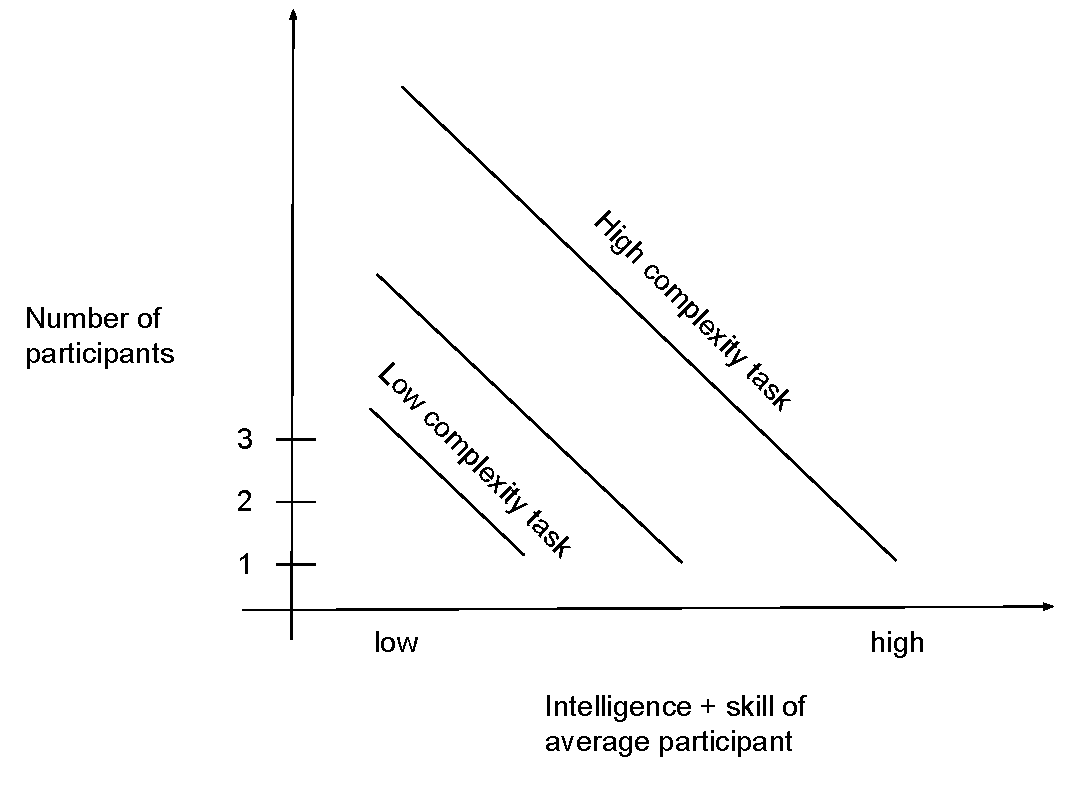
\includegraphics[width=0.8\textwidth]{images/people-per-task-for-skill-level.pdf}
\caption{Three levels of task complexity are shown. As task complexity increases, the size of the team needs to grow. The growth may be less if the team members are brilliant. Those brilliant people cost more and there are fewer of them available.}
\end{figure}

\subsection{Why is bureaucracy so hard?}

When a person has a positive experience engaging with bureaucracy, positive attribution is made to the people involved. Or ease of a solution makes the bureaucracy less visible and the solution seems obvious. 

When a person has a negative experience with bureaucracy, complaints are about the incompetence of the people involved, or the incomprehensibleness of the system. Don't these bureaucrats know how to do their job? Why isn't the solution obvious? Why does this system not work for me?

many nuances not visible to external perspective
\begin{itemize}
    \item organization politics (personalities, resources, prioritization)
\item lack of unified voice
\item legacy policies to overcome/change/be consistent with
\end{itemize}




\subsection{Hierarchy of Roles\label{sec:hierarchy_of_roles}}

Ideally sufficient depth and breath for decision making would be embodied in one person. That might not be possible in every situation. One way to resolve this is to identify distinct scopes of responsibility and then assign different members of an organization separate scopes for decision making. Within a decision making scope there may be more work than one person can handle, so a team is formed. That team may have some members focused on tactical work and other members focused on strategy and coordination. Hierarchy within an organization is the formalization of separate decision-making scopes and associated specialization. 

Partitioning knowledge and decision making enables complexity beyond what one person can accomplish and causes friction among members. An expert reporting to a manager knows things the manager does not, and the manager may have context that the expert lacks. Both bureaucrats (the expert and the manager) need to convey their respective nuance and seek out the holistic view.

A hierarchical organization with partitioned knowledge introduces a challenge: the order in which you share information with others matters. Your choices for who to first describe an idea to are your peers, your management, and your subordinates. \marginpar{[Tag] Trilemma} The people subordinate to you know more about the topic and are exposed to the consequences. Giving them a chance to vet the idea results in a more robust idea and validates their value in organization. Sharing your idea with management first allows your superiors to provide context you might not be aware off. Starting the conversation with your peers first indicates you value the relationship and decrease the risk of overlapping work.

\ \\

Although I've included hierarchy in the section on Fundamentals of Bureaucracy, I don't mean to imply that hierarchy is a required feature of bureaucracy. Hierarchies of bureaucrats are a common \href{https://en.wikipedia.org/wiki/Organizational_structure}{organizational structure} and therefore worthy studying even if not essential to bureaucracy. The relevance of understanding hierarchy is to identify recurring behavior and patterns to leverage.
Organizations of bureaucrats can intentionally work against hierarchy, but the amount of effort needed to enable alternatives implies that hierarchy is a natural approach.

The benefits of formal hierarchy include improved capacity for the number of policy decision made, enabling consistency of decisions, and leveraging specialization of knowledge. 
Hierarchical decision making has costs: higher latency, inconsistency among bureaucrats, waste due to inefficiency, and many others described in \S\ref{sec:unavoidable_hazards}. As another example of harm, hierarchy enables strategic ignorance. Bureaucrats in positions of power can deny having knowledge of improper activity. 
\footnote{L.~McGoey, ``The Unknowers: How Strategic Ignorance Rules the World" (2019)
% review: https://www.tandfonline.com/doi/abs/10.1080/19460171.2020.1768422?journalCode=rcps20
and 
L.~McGoey, ``The logic of strategic ignorance" (2012). DOI 
10.1111/j.1468-4446.2012.01424.x
}


The structure of an organization is dynamic, but at each point in time an organization typically has a defined set of roles. Each role is distinguished by different scopes of decision authority. 




Roles in an organization are defined by the boundaries of responsibility. The purpose of a role is to minimize conflict and reduce redundancy, allowing control. Clear responsibility enables effective bureaucracy. 


A conventional characterization of an organization's hierarchy involves two criteria: the depth and breadth of the org chart.
The more people a supervisor oversees, the flatter the organization -- that's the breadth of the organization. See the Valve handbook \cite{2012_Valve} and Joreen's essay \cite{1972_Joreen} for contrasting views on the shape of an organization's hierarchy. Depth of the hierarchy is how many layers there are.

A more practical view of an organization's hierarchy also involves two criteria. The two choices in how a hierarchy is shaped are 
1) how many people a supervisor oversees and 
2) how many supervisors a person has. 
Though you might naively expect that an employee has one boss, but that is \href{https://en.wikipedia.org/wiki/Matrix_management}{not a requirement}. A supervisor for a given topic may have many people reporting to them, and a bureaucrat with multiple roles may report to more than one supervisor.

\ \\

Acting as part of a group means ceding part of your autonomy. Hierarchy is an additional layer of ceding responsibility and adding expectations about relationships.
The consequence of hierarchy in an organization means that as a member of the bureaucracy you do not have full autonomy -- otherwise you would not be a member of the hierarchy. At the same time you are not under strict control of the organization -- you still have some subjective decision making authority as a bureaucrat.

The person at the top of the hierarchy does not know everything. The person at the top of the hierarchy does not have input on every decision made in the organization. Some autonomy is retained by all members of the bureaucracy.

Independent of the defined roles and designated titles in an organization's hierarchy, there are a set of implicit roles and a separate social hierarchy of informal influencers and decision makers. Informal influencers in a bureaucracy usually have long relationships with the decision maker or relevant credentials or both. The credentials can be formal (e.g., a \href{https://en.wikipedia.org/wiki/Doctor_of_Philosophy}{PhD}) or informal (demonstrated success on a project). In either case, the decision maker is relying on another person's expertise. 

Another set of informal relations within an organization is mentors and mentees. These relations allow mentors to transmit institutional knowledge to mentees, and allows people in senior positions to access the novice perspective. 


\ \\

One consequence of hierarchy is a sense of fear felt by people who report to other people. This fear stems from the loss of control (less autonomy) that leaves the person feeling disempowered. 

For example, consider the following relationship. A person, Sue, is perceived to have power over another person, Amy, because Amy gave up some control to Sue. Amy not having control triggers the feeling of fear in Amy, regardless of how Sue behaves. 

If Sue is aware of the potential for this emotional experience, Sue can compensate for Amy's fear by being friendly and receptive towards Amy. Alternatively Sue may exploit or rely on the fear felt by subordinates. 


% Active bystander when the person doing wrong is in a position of authority
% PACT (Probe, Alert, Challenge, Take Action)
% https://mobile.twitter.com/GeorgetownABLE/status/1408498438203969541


% Mintzberg's Coordination Mechanisms
% https://www.youtube.com/watch?v=IZET8VjSifQ


\subsection{Organizational chart as a guide and a lie}

An \href{https://en.wikipedia.org/wiki/Organizational_chart}{organizational chart} (hereafter ``org chart'') identifies roles and the relations among roles. An org chart is at best a snapshot in time, and more often aspirational than descriptive. In spite of possible deficiencies, an org chart helps outsiders and newcomers understand the scope of responsibilities and interactions.\footnote{The organization chart hasn't always existed. The \href{https://en.wikipedia.org/wiki/George_Holt_Henshaw\#First_organization_chart}{first known org chart} was created in the 1850s.}

Org charts are a lie in the sense that undocumented relationships can matter more than the roles. Org charts fail to capture the informal roles that facilitate progress in any organization. 

Org charts foster a lie by creating sense power dynamics based on visual orientation. For more on this issue see \S~\ref{org-chart-orientation}.



\subsection{Approval process}
\subsection{Meetings for coordination}
coordination and signaling
\subsection{Written communication}
Reports, memos, emails are artifacts of bureaucracy. They create evidence and can be used for good or bad. 


\section{History of Bureaucracy}

I'm mostly going to skip history and merely cite other scholarly references


https://en.wikipedia.org/wiki/Bureaucracy

\section{Scope}

\subsection{scale}
Although bureaucracy can be present for one person, and bureaucracy is often apparent on teams (e.g., 3 to 20 people), this book primarily focuses on the situation of multiple teams comprising an organization. This might be a few hundred people (above \href{https://en.wikipedia.org/wiki/Dunbar's_number}{Dunbar's number}) up to millions of people. 

There are tens of companies that employ more than a million people [see \href{https://en.wikipedia.org/wiki/List_of_largest_employers}{Wikipedia's list of largest employers}], including Walmart, Amazon, and McDonald's.

Small companies and non-profit organization also encounter bureaucracy. The complexity of the tasks may be different, but the same scale-independent patterns can emerge because of a common factor: human behavior.

\chapter{Bureaucracy throughout life}
\section{Avoiding Bureaucracy is Nearly Impossible}

The only situation where bureaucracy might not exist is if you live completely on your own, with no interaction with other people. That means completely disengaging from society. Even then, personal routines are a self-imposed form of bureaucracy, with the roles of policy maker, bureaucrat, and subject collapsed to a single person -- you.

Self-sufficiency and autonomy are attractive alternatives bureaucracy. The way participants in modern society strive for self-sufficiency is by denying their dependence on modern society. That's a relabeling of selfishness which feels better. 

For the rest of us who operate as members of a society, bureaucracy is necessary for our rights. We prove our name by cooperating with other people, and our name helps us claim our citizenship. That's a subjective policy that \glspl{stakeholder} in society agree to. 



The specific way a society is constructed (democratic, authoritarian, dictatorship, anarchy) is irrelevant -- bureaucracy is still present. Even the libertarian view of relying on contract enforcement implies some amount of bureaucracy (e.g., forums for resolving contract disputes like a court system). 


Not all bureaucracy is due to the state, nor is bureaucracy confined to companies. Parenting involves coming up with situation-specific requirements for children, with the organization being the family as mentioned in \S\ref{sec:bureaucracy-early-childhood}. Dress codes for sports teams are arbitrary standards. 
Store clerks are bureaucrats, as are website forum moderators.  Content moderation is the process of (inconsistently) enforcing arbitrary standards. This mindset even permeates individuals as internalized expectations of policy and enforcement when no one else is present. 

Recognizing instances of bureaucracy enables more skillful interaction, whether as a bureaucrat or as a subject. The remainder of this section  illustrates both the view of a person interacting with bureaucracy as a \gls{subject}, and the perspective of bureaucrats working within organizations. 






\section{Beginnings and Endings}
In life there are some standard milestones: birth, education, work, death. Each of those milestones corresponds to engaging bureaucracy. 

Within the employment phase, there are pairs start and end events which may apply: hiring or getting hired; firing, getting fired, or quitting. 



\section{Relationships throughout life}
In the conventional Western progression, relationships include
\begin{itemize}
    \item pre-education childhood: primarily family, possible community members, caretakers
    \item primary education: family, friends, teachers
    \item college, graduate school: friends, teachers, advisors
    \item employment: managers above you, peer employees, people you manage
    \item healthcare
\end{itemize}

\subsection{school vs business}
School (high school, undergraduate, graduate school) is  different from working in a large organization. 


\subsection{undergrad vs graduate}
 education process roles and expectations vary over time

\subsection{military}
Less than 0.5\% of the United States population serves in the military. \footnote{source: \href{https://www.cfr.org/backgrounder/demographics-us-military}{Council on Foreign Relations}}

The military, with rigid hierarchy and defined protocols, is also a distinct experience. 


% education process

% healthcare

\chapter{Bureaucracies are made of Humans}
% an insider's perspective
% unordered essays to be clustered latter

\subsubsection{Organization chart orientation
\label{org-chart-orientation}}

A common method of describing relations within the bureaucracy is the organization chart (colloquially, the ``org chart"). Normally the CEO is at the top of the chart, middle management is in the middle, and managed employees are at the bottom. See figure~\ref{org_chart_orientation_ceo-at-top} 


An organization's culture is subtly conveyed by artifacts like org charts. 
% What's the point of this section? Is there a consequence, or is this just an observation?
There are emotional connotations to alternative layouts. You can alter expected relations (culture and norms) by playing with orientation of the org chart.
Org chart orientation can be overanalyzed, so this exploration is limited.

The point of thinking about org chart orientation is to frame how you perceive your supervisors, peers, subordinates. Notice that the framing is embedded in the words -- prefixes super (over) and sub (under). 
These concepts inform what you expect from relations.
Do I seek support or direction and guidance from my boss? What do I expect from my boss, peers subordinates? What do I expect to provide them?

%\begin{itemize}
%\item 
%\end{itemize}

The relative orientation of the \href{https://en.wikipedia.org/wiki/Chief_executive_officer}{CEO} to workers sets expectations for relations. 
Options for orientation are the conventional CEO at top
(figure~\ref{org_chart_orientation_ceo-at-top}), 
CEO at the bottom (figure~\ref{org_chart_orientation_ceo-at-bottom}),
CEO on the right (figure~\ref{org_chart_orientation_ceo-leads}),
CEO on the left (figure~\ref{org_chart_orientation_ceo-follows}),
CEO as the center of a star 
(Example: \href{https://en.wikipedia.org/wiki/File:League_of_Nations_Organization.png}{League of Nations diagram})

\begin{figure}
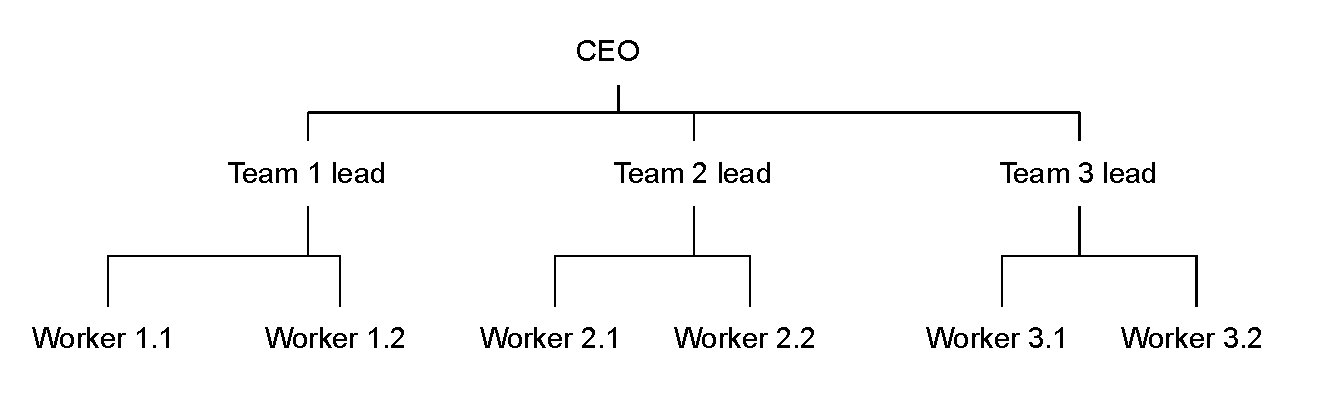
\includegraphics[width=1\textwidth]{images/org-chart-orientation-ceo-at-top.pdf}
\caption{Standard orientation. Role with most responsibility and authority is at top. Left-right ordering is intended to be irrelevant in this view, though left-to-right reading order emphasizes importance.}
\label{org_chart_orientation_ceo-at-top}
\end{figure}

\begin{figure}
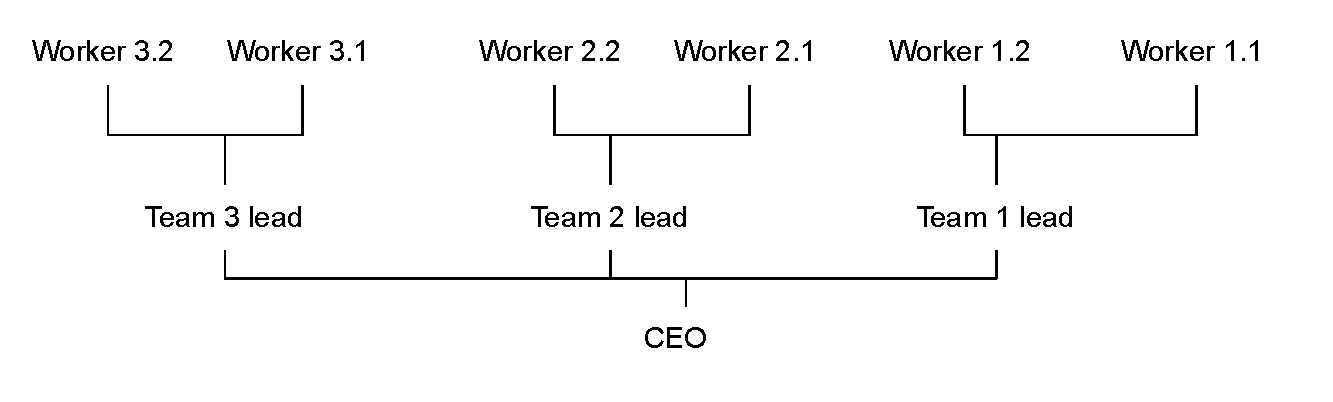
\includegraphics[width=1\textwidth]{images/org-chart-orientation-ceo-at-bottom.pdf}
\caption{Flipping the orientation presents a more realistic view of the CEO's responsibility. The crushing burden of servant leadership is clear. Left-right ordering is intended to be irrelevant in this view.}
\label{org_chart_orientation_ceo-at-bottom}
\end{figure}

\begin{figure}
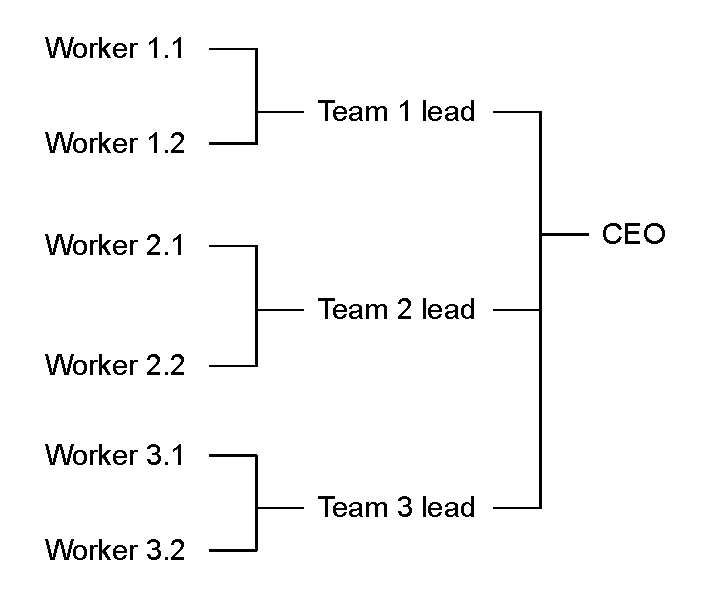
\includegraphics[width=0.8\textwidth]{images/org-chart-orientation-ceo-leads.pdf}
\caption{Conventionally time flows from left (old) to right (new), so in this graph the CEO leads the charge into the unknown. Is the CEO dragging workers forward, or are the workers pushing the CEO? The top-to-bottom ordering can be read as importance. }
\label{org_chart_orientation_ceo-leads}
\end{figure}

\begin{figure}
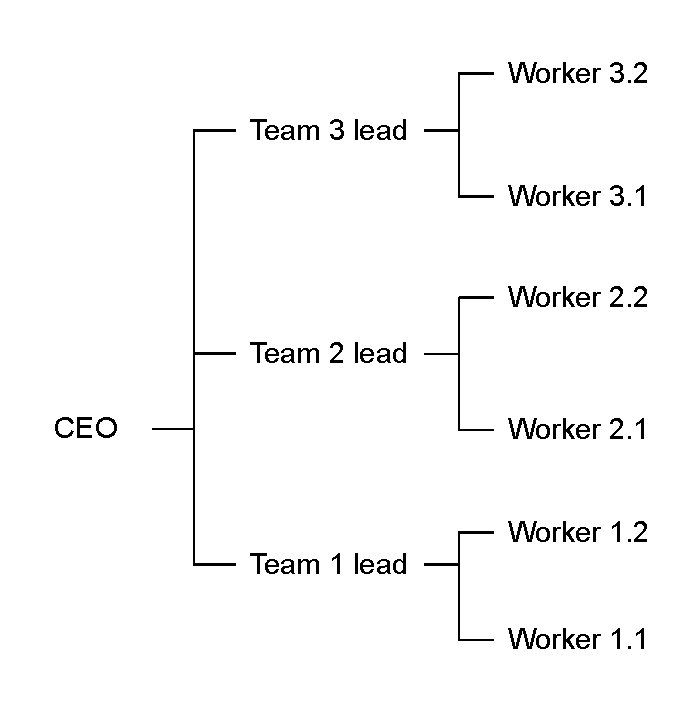
\includegraphics[width=0.8\textwidth]{images/org-chart-orientation-workers-lead.pdf}
\caption{The ``chariot view'' with the CEO in the chariot and the workers out front. Workers are in the future, the CEO is in the past operating on old information. As with figure~\ref{org_chart_orientation_ceo-leads}, top-to-bottom ordering can be read as importance. }
\label{org_chart_orientation_ceo-follows}
\end{figure}



%extension of 
% \href{https://en.wikipedia.org/wiki/Conway\%27s_law}{Conway's law}: seating chart reflects org chart

% https://graphthinking.blogspot.com/2020/05/invisible-bureaucracy.html

\subsection{Social and Bureaucratic interactions}

Interactions with other people in an organization are either social interaction or bureaucratic interaction. 

As examples of each of these,
\begin{itemize}
\item Social interaction example: "Did you see the game on TV last night? Our team really did well, right? I thought about getting tickets for the game but they were sold out."
\item Bureaucratic interaction example: "You'll need to get approval from Sue before presenting your idea to the board for their review. Then talk with Russ and get his thoughts."
\end{itemize}
Both social and bureaucratic interactions are vital to cohesion in an organization of people. 


Bureaucratic interaction can be broken into two subcategories: \gls{visible bureaucracy} (procedures and processes are written down and can be discovered by stakeholders)  and \gls{invisible bureaucracy} (procedures and processes are known to some stakeholders and are conveyed verbally to some of the other stakeholders).

Invisible bureaucracy is akin to invisible domestic or relation work outside the professional environment. The work associated with emotional cohesion, logistics, planning, scheduling, and communicating is hard to quantify so it does not get counted.

To make invisible work and invisible bureaucracy visible, document the work.


The relevance of this jargon is to break down the components of an organization's "culture" experienced by participants. The ratio of social/visible bureaucracy/invisible bureaucracy is a characterization of the culture. There are norms associated with each of these three categories.
essential bureaucracy is the minimum necessary to address the complexity of the problem space. This is tricky since the optimization can be with respect to resilience to change, resilence to edge cases, staff turn-over, speed experienced by consumer, financial cost, organization time, organization staffing level.

Undesirable bureaucracy is either accidental or legacy
% https://graphthinking.blogspot.com/2021/02/how-to-have-efficient-bureaucracy.html

In an ideal scenario with no bureaucracy, everyone comes to the same conclusion when presented with the same information. Then the management process of building consensus becomes unnecessary. There is no need to fight over resources (money, staffing) and no need to fight over direction.

While that ideal scenario is not going to happen, it points to how to improve bureaucratic efficiency:
\begin{itemize}
\item each person has the same information. 
\item each person applies the same decision making process consistently
\item every person has the same incentives
\end{itemize}
The reason bureaucracy is inefficient is
\begin{itemize}
\item not everyone has the same information
\item processes are inconsistent
\item incentives vary
\end{itemize}
Also, add the issue that each person's reference experiences are unique. As a consequence, decision making is subjective. 

Can any action be taken to improve bureaucratic efficiency? Yes!
\begin{itemize}
\item you can share information with other stakeholders
\item you can seek information from other stakeholders
\item you can strive for and demonstrate transparency
\item apply consistent processes 
\item hold others (and yourself) accountable 
\item account for varying incentives and reference experiences
\end{itemize}

\subsection{Motivation of Bureaucrats}

To understand the bureaucrats you work with, appreciating their diverse motives is instructive. If you expect everyone to have the same motives as you, then you will be surprised by the friction. 

Motivations of participants are rarely ``how can I make the company more successful" or even ``how can I sell/produce more product"? Usually motivation is based on personal success in various manifestations, which leads to emergent phenomena which appears confounding to observers outside the bureaucracy. 


% see https://en.wikipedia.org/wiki/Social_influence

Each bureaucrat has a motive, even the bureaucrats who do nothing. 
% https://graphthinking.blogspot.com/2020/02/there-is-no-idle-status-for-paid.html
In an organization where you are a paid bureaucrat, you are either actively working for improvement of the organization, or your existence is parasitic to the organization. There is no ``idle" status for paid employees in an organization with limited resources.

Not too efficient such that I eliminate the need for my job, and not so inefficient that the organization fails and I lose my job. Increasing the efficiency of bureaucracy is good for the organization and the outcomes, but can be harmful to the bureaucrat's career.

Career stability within an organization is a benefit, and it can be leveraged to take more risk. However, it typically manifests as inaction by an employee. There's no harm to the employee in not taking action. If an employee doesn't do anything, nothing bad will happen to that employee. Career stability decreases extrinsic motivation.



Example motivations for bureaucrats: stability, money, travel, problem solving, like being associated with org, logistical convenience (``the office is near where I lived.'')


% https://graphthinking.blogspot.com/2021/04/laffer-curve-and-minimum-viable.html

The Laffer curve is a claim in economics that there is a relation between government tax rates and the revenue from taxes collected. The relation, based on Rolle's theorem, says that between a tax rate of 0% and 100%, there must be some amount of tax that corresponds to the maximum of revenue. 

While the mathematical statement may be provable, the use in economics seems hand-wavy. In this post, I'll extend that hand-waviness to a different domain: bureaucratic processes in organizations. The relation to the Laffer curve is that bureaucratic processes a tax on productivity. 
\section{Bureaucratic Fallacies\label{sec:fallacies}}

There are perspectives that are \gls{thought terminating}. Identifying these enables you to understand both why they are attractive and how they are incomplete.

See also unavoidable hazards in \S~\ref{sec:unavoidable_hazards}.

\ \\

\textit{Bureaucratic fallacy}: \textbf{Bureaucracy is bad}. \\
\textit{Why this feels true}: when a person subjected to bureaucracy has a negative experience, the easiest attribution is to the least-understood aspect -- the bureaucracy.\\
\textit{What this is missing}: \Gls{bureaucracy} is neither good nor bad. 

\ \\

\textit{Bureaucratic fallacy}: \textbf{There is no point in planning ahead since everything (staffing, funding, purpose, scope) is always changing.}\\
\textit{Why this feels true}: Change can feel disorienting, especially when it is unexpected. \\
\textit{What this is missing}: Preparing for change and thinking ahead about contingencies enables effective use of resources. Have a vision and work towards it while accounting for change. 


\ \\

\textit{Bureaucratic fallacy}: \textbf{Bureaucracy is an aberration, a mistake, due to poor planning or incompetent participants}. \\
\textit{Why this feels true}: TODO\\
\textit{What this is missing}: TODO

\ \\

\textit{Bureaucratic fallacy}: \textbf{Bureaucracy is inefficient}. \\
\textit{Why this feels true}: Expressed by both subjects and bureaucrats who observe seemingly wasteful processes.\\
\textit{What this is missing}: If bureaucracy were truly inefficient (not allocating resources in the most efficient way), then it would be replaced by a more efficient approach. The key is to ask, ``efficient with respect to what metric?'' The metric of money, time, number of people, stability, robustness to perturbation.  Second, what would motivate improved efficiency? Without incentives, change is less likely. 

\ \\

\textit{Bureaucratic fallacy}: \textbf{Bureaucracy is due to malfeasance.}\\
The specific number of malicious bureaucrats ranges from ``all of the participants'' to ``just enough to be problematic.'' \\
\textit{Why this feels true}: There are bad actors. 
\textit{What this is missing}: Bureaucracy is unavoidable, and most of the participants are earnestly trying to help or are not making a positive contribution. Processes within bureaucracy are used to deal with malicious bureaucrats, like isolation or promotion. 

\ \\

\textit{Bureaucratic fallacy}: \textbf{Bureaucracy is a sign of decay from within the org.} \\
\textit{Why this feels true}: TODO\\
\textit{What this is missing}: Bureaucracy is unavoidable emergence in any/every organization.

\ \\

\textit{Bureaucratic Fallacy}: \textbf{If this request can't be expedited, it must not be important}.  \\
\textit{Why this feels true}: Other people would demonstrate they care about what I am working on by prioritizing things I am dependent on.
\textit{What this is missing}: When everything gets prioritized, that's the same as nothing getting priority.

\ \\

\textit{Bureaucratic Fallacy}: \textbf{Duration of a task is how long it would take one person to accomplish}.  \\
\textit{Why this feels true}: TODO\\
\textit{What this is missing}: Fails to account for the overhead of interaction and delays due to asynchronous engagement.


\ \\

% https://graphthinking.blogspot.com/2019/08/two-misleading-simplifications-when.html
\textit{Bureaucratic Fallacy}: \textbf{Consider the average or majority (to the exclusion of outliers)}. \\
Why this simplification is misleading: For sufficiently large ensembles, the outliers alter the outcome. The larger the ensemble, the more significant the role of the outlier minority.

\ \\

\textit{Bureaucratic Fallacy}: \textbf{people learn from their mistakes}. \\
\textit{Why this feels true}: TODO\\
\textit{What this is missing}: Requires a low latency feedback loop and incentive to change.

\ \\

\textit{Bureaucratic Fallacy}: \textbf{processes are serial}.\\
\textit{Why this feels true}: TODO \\
\textit{What this is missing}: TODO


\ \\

\textit{Bureaucratic Fallacy}: \textbf{Hard work creates results}.\\
\textit{Why this feels true}: TODO\\
\textit{What this is missing}: TODO


\ \\

\textit{Bureaucratic Fallacy}: \textbf{Motivations for bureaucrats are categorized as individualistic, tribal, organizational, societal, or humanity}.\\
\textit{Why this feels true}: TODO\\
\textit{What this is missing}: TODO


\ \\

\textit{Bureaucratic Fallacy}: 
\textbf{you cannot pay a little and get a lot}; see \href{https://en.wikipedia.org/wiki/Common_law_of_business_balance}{Common law of business balance}. \\
\textit{Why this feels true}: TODO\\
\textit{What this is missing}: This doesn't allow for creative solutions and ignores \href{https://en.wikipedia.org/wiki/Nudge_theory}{nudge theory} from behavioral economics. 


\subsection{Hiring into a Bureaucracy}

Hiring shapes the culture of an organization and determines what is feasible, both by the skills of those hired and how well new hires integrate with the existing organization. 

Hiring is an expensive process in terms of money, time, emotional investment of candidates, and the burden of reviewing applicants. 
% SO WHAT? What's the consequence?

When hiring into an organization there is a selection bias in the people who join a bureaucracy, and there is a selection bias who stays in bureaucracy. 
% SO WHAT? What's the consequence?



Regardless of the specifics of the job, there are specific attributes that make a candidate more likely to be successful in a bureaucracy. In addition to role-specific skills, hire for \href{https://en.wikipedia.org/wiki/Metacognition}{metacognition}, social skills, and intrinsic motivation.

% https://graphthinking.blogspot.com/2021/04/screening-for-metacognition-in-job.html

% https://graphthinking.blogspot.com/2021/07/screening-for-intellectual-empathy-in.html

% https://graphthinking.blogspot.com/2021/04/questions-to-ask-interviewer-when.html



% reputation management; building and spending political capital

% product deployment internal to the org

% intra- and inter- team dynamics
% https://graphthinking.blogspot.com/2021/07/patterns-anti-patterns-in-bureaucracy.html

% intra- and inter- team dynamics

\section{Teams as a subdivsion of an Organization}

In the context of altering teams, there are a few major levers available: create new team, merge teams, dissolve a team. 

For a given set of teams, the lateral interactions are competitive or cooperative. Coordination is required (or conflict will occur) for money, staffing, and resources. Examples of resources include access to or control of data, computer equipment, hardware, floor space, prestige, products (output)

% homogeneity of intelligence of members in an organization; percolation theory of cowboys

% professional training

% conferences 
% presenting
% audience
% socializing


\clearpage

\printglossaries

\nocite{*} % causes LaTeX to include every entry in your .bib file.
\bibliographystyle{plain-annote}
\bibliography{biblio}

\end{document}
